\section{Theoretical Analysis}
\label{sec:analysis}

In this section, the circuit shown in Figure~\ref{fig:circuit} is analysed
theoretically, in terms of its time and frequency responses.

\subsection{Mesh Analysis}

\begin{figure}[h!] \centering
	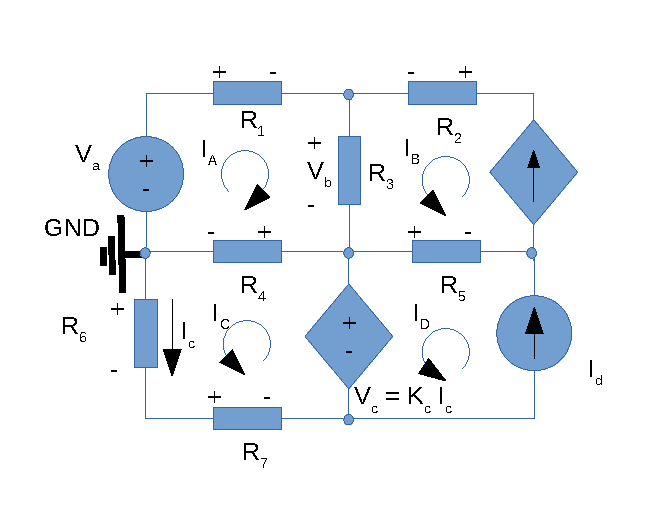
\includegraphics[width=0.7\linewidth]{circ_mesh.pdf}
	\caption{Mesh Analysis}
	\label{fig:circuitMesh}
\end{figure}

The Figure~\ref{fig:circuitMesh} has both the mesh's currents and the 
component's admited direction.
This reference is indispensable for the Mesh Analysis.
Using KVL in each of the 4 meshes, we achieve the following equations:
\vspace{0.5cm}

Malha A:
$$ R_1 * I_A + R_3(I_A+I_B) + R_4(I_A+I_C) = V_A$$

Malha B:
$$ I_B = K_c * R_3(I_A + I_B) $$

Malha C:
$$ R_4(I_A + I_C) + R_6 * I_C + R_7 * I_C = K_c * I_C $$

Malha D:
$$ I_D = I_d $$

\vspace{0.5cm}

After doing some algebra, we can get the following system of equations. After that, 
we can solve it by enquadrating it in a matriz like shown bellow:

\vspace{0.5cm}

\[
\begin{bmatrix}
R_1 + R_3 + R_4 & R_3 & R_4 & 0\\
K_b * R_3 & K_b * R_3 - 1 & 0 & 0\\
R_4 & 0 & R_6 - K_c + R_7 - R_4 & 0\\
0 & 0 & 0 & 1\\
\end{bmatrix}
\cdot
\begin{bmatrix}
I_A\\
I_B\\
I_C\\
I_D\\
\end{bmatrix}
=
\begin{bmatrix}
V_a\\
0\\
0\\
I_d\\
\end{bmatrix}
\]

\vspace{0.5cm}

After solving these equations using octave, we get 
the following results:

\vspace{0.5cm}

\csvautotabular{../mat/malhas.txt}

\vspace{0.5cm}

To get the current in each resistor, we use the following equations:

\vspace{0.5cm}

$$ I_1 = I_A $$
$$ I_2 = I_B $$
$$ I_3 = I_A + I_B $$
$$ I_4 = I_A + I_C $$
$$ I_5 = I_B - I_D $$
$$ I_6 = I_C $$
$$ I_7 = I_C $$

\vspace{0.5cm}

Leading to the results bellow:

\vspace{0.5cm}

\csvautotabular{../mat/cur.txt}

\vspace{1.0cm}

\newpage

\subsection{Nodal Analysis}

\vspace{0.5cm}

\begin{figure}[h!] \centering
	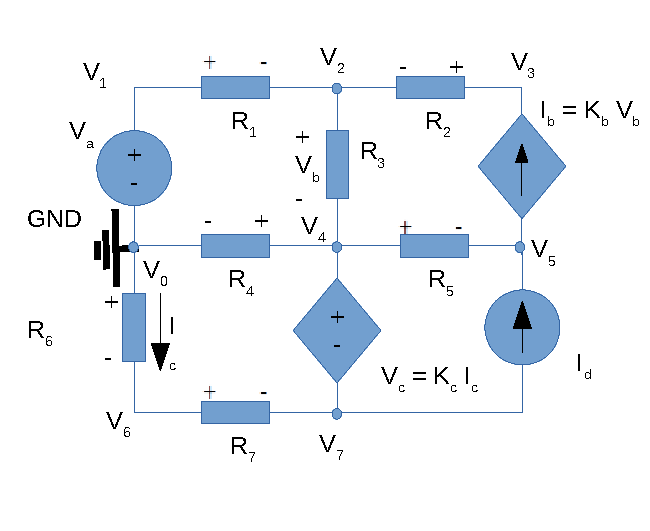
\includegraphics[width=0.7\linewidth]{circ_node.pdf}
	\caption{Nodal Analysis}
	\label{fig:circuitNodes}
\end{figure}

\vspace{0.5cm}

The Figure~\ref{fig:circuitNodes} has the node references appended.
This reference is indispensable for the Nodal Analysis.
Using KVL in each of the 4 meshes, we achieve the following equations:

\vspace{0.5cm}

Node 2:
$$ (V_1 - V_2)G_1 + (V_3 - V_2)G_2 = (V_2 - V_4)G_3 $$

Node 3:
$$ (V_3 - V_2)G_2 = K_b(V_2 - V_4) $$

Node 5:
$$ (V_4 - V_5)G_5 + I_d = K_b(V_2 - V_4) $$

Node 6:
$$ (V_0 - V_6)G_6 = (V_6 - V_7)G_7 $$

Additional equations:
$$ V_0 = 0 $$
$$ (V_1 - V_0) = V_a $$
$$ V_4 - V_7 = K_c(V_0 - V_6)G_6$$
$$ (V_0 -V_6)G_6 - (V_4 - V_0)G_4 + (V_1 - V_2)G_1 = 0 $$

\vspace{0.5cm}

Similarly to the last example, the algebric manipulation brings us to the following system of equations, 
and the solution can be found by enquadrating it in a matriz like shown bellow:

\[
\begin{bmatrix}
1 & 0 & 0 & 0 & 0 & 0 & 0\\
0 & 0 & 0 & 1 & 0 & K_c * G_6 & -1\\
G_1 & -G_1-G_2 - G_3 & G_2 & G_3 & 0 & 0 & 0\\
0 & -K_b & 0 & G_5 + K_b & -G_5 & 0 & 0\\
0 & -K_b & 0 & G_5 + K_b & -G_5 & 0 & 0\\
0 & 0 & 0 & 0 & 0 & -G_6-G_7 & G_7\\
G_1 & -G_1 & 0 & -G_4 & 0 & -G_6 & 0\\
\end{bmatrix}
\cdot
\begin{bmatrix}
V_1\\
V_2\\
V_3\\
V_4\\
V_5\\
V_6\\
V_7\\
\end{bmatrix}
=
\begin{bmatrix}
V_a\\
0\\
0\\
0\\
-I_d\\
0\\
0\\
\end{bmatrix}
\]

\vspace{0.5cm}

After solving these equations using octave, we get 
the following results:

\vspace{0.5cm}

\csvautotabular{../mat/nos.txt}

\vspace{1.0cm}

\subsection{Result Comparison }

In order to compare the awnsers from the mesh and node methods, we
can use the voltage values we obtained and, using Ohm's law ~(\ref{eq:ohm}), check if the
current values are similar.

\vspace{0.5cm}

\begin{equation}
  U = RI.
  \label{eq:ohm}
\end{equation}

\vspace{0.5cm}

\csvautotabular{../mat/comp.txt}

\vspace{0.5cm}

The interpretation of the previous table leads us to the conclusion that the
values are virtualy equal.

\vspace{0.5cm}
